
%\documentclass[11pts,a4paper,amsmath,amssymb,floatfix]{article}%{report}%{book}
\documentclass[12pts,a4paper,amsmath,amssymb,floatfix]{article}%{report}%{book}
\usepackage[pdftex,colorlinks=true,urlcolor=blue,citecolor=blue]{hyperref}
\usepackage{graphicx} 
\usepackage{wrapfig,pdfpages}% Include figure files
%\usepackage{dcolumn,enumerate}% Align table columns on decimal point
\usepackage{enumerate}%,enumitem}% Align table columns on decimal point
\usepackage{bm,dpfloat}% bold math
%\usepackage[pdftex,bookmarks,colorlinks=true,urlcolor=rltblue,citecolor=blue]{hyperref}
\usepackage{amsfonts,amsmath,amssymb,stmaryrd,indentfirst}
\usepackage{times,psfrag}
\usepackage{natbib}
\usepackage{color}
\usepackage{units}
\usepackage{rotating}
\usepackage{multirow}

%%% For restarting section numbering
\makeatletter
\@addtoreset{section}{part}
\def\@part[#1]#2{%
    \ifnum \c@secnumdepth >\m@ne
      \refstepcounter{part}%
      \addcontentsline{toc}{part}{\thepart\hspace{1em}#1}%
    \else
      \addcontentsline{toc}{part}{#1}%
    \fi
    {\parindent \z@ \raggedright
     \interlinepenalty \@M
     \normalfont\centering
     \ifnum \c@secnumdepth >\m@ne
       \LARGE\bfseries \partname\nobreakspace\thepart
       \par\nobreak
     \fi
     \huge \bfseries #2%
     \markboth{}{}\par}%
    \nobreak
    \vskip 3ex
    \@afterheading}
\renewcommand\partname{Part}
\makeatother



\usepackage{pifont}
\usepackage{subfigure}
\usepackage{subeqnarray}
\usepackage{ifthen}

\usepackage{supertabular}
\usepackage{moreverb}
\usepackage{listings}
\usepackage{palatino}
%\usepackage{doi}
\usepackage{longtable}
\usepackage{float}
\usepackage{perpage}
\MakeSorted{figure}
%\usepackage{pdflscape}
\usepackage{soul} %% use \hl to higlight text

\usepackage{framed}
\definecolor{shadecolor}{gray}{0.9}
%\usepackage{booktabs}
%\newcommand{\ra}[1]{\renewcommand{\arraystretch}{#1}}


\definecolor{rltblue}{rgb}{0,0,0.75}


%\usepackage{natbib}
\usepackage{fancyhdr} %%%%
\pagestyle{fancy}%%%%
% with this we ensure that the chapter and section
% headings are in lowercase
%%%%\renewcommand{\chaptermark}[1]{\markboth{#1}{}}
\renewcommand{\sectionmark}[1]{\markright{\thesection\ #1}}
\fancyhf{} %delete the current section for header and footer
\fancyhead[LE,RO]{\bfseries\thepage}
\fancyhead[LO]{\bfseries\rightmark}
\fancyhead[RE]{\bfseries\leftmark}
\renewcommand{\headrulewidth}{0.5pt}
% make space for the rule
\fancypagestyle{plain}{%
\fancyhead{} %get rid of the headers on plain pages
\renewcommand{\headrulewidth}{0pt} % and the line
}

\def\newblock{\hskip .11em plus .33em minus .07em}
\usepackage{color}

%\usepackage{makeidx}
%\makeindex

\setlength\textwidth      {16.cm}
\setlength\textheight     {22.6cm}
\setlength\oddsidemargin  {-0.3cm}
\setlength\evensidemargin {0.3cm}

\setlength\headheight{14.49998pt}
\setlength\topmargin{0.0cm}
\setlength\headsep{1.cm}
\setlength\footskip{1.cm}
\setlength\parskip{0pt}
\setlength\parindent{0pt}


%%%
%%% Headers and Footers
\lhead[] {\text{\small{EG501V -- Computational Fluid Dynamics}}}
\rhead[\text{\small{Assignment 2017/18}}]{Assignment 2017/18}
\lfoot[]{CFD}
\rfoot[\thepage]{\thepage}
\renewcommand{\headrulewidth}{0.8pt}


%%%
%%% space between lines
%%%
\renewcommand{\baselinestretch}{1.5}

\newcommand{\frc}{\displaystyle\frac}
\newcommand{\red}{\textcolor{red}}
\newcommand{\blue}{\textcolor{blue}}
\newcommand{\green}{\textcolor{green}}
\newcommand{\purple}{\textcolor{purple}}
\newcommand\Rey{\mbox{\textit{Re}}\,\,}
\newcommand\bfr[1]{\textcolor[rgb]{1,0.00,0.00}{\textbf{\textsf{#1}}}}
\newcommand\ra{$\rightarrow$}
\newcommand\cm{\textcolor[rgb]{0.00,0.50,0.00}{\checkmark}\,\,}


%%%%%%%%%%%%%%%%%%%%%%%%%%%%%%%%%%%%%%%%%%%
%%%%%%                              %%%%%%%
%%%%%% END OF THE NOTATION SECTION  %%%%%%%
%%%%%%                              %%%%%%%
%%%%%%%%%%%%%%%%%%%%%%%%%%%%%%%%%%%%%%%%%%%


% Cause numbering of subsubsections.
%\setcounter{secnumdepth}{8}
%\setcounter{tocdepth}{8}

\setcounter{secnumdepth}{4}%
\setcounter{tocdepth}{4}%


\begin{document}

\section{Introduction}
High-density polyethylene (HDPE) is the third largest commodity plastic material produced in the world (after PVC and PP) with annual production of 51.33 MMT (2016) and worth of approximately USD 64 billions. HDPE resin is used in a wide range of applications from food and beverage packaging to corrosion- and thermal-resistant pipes. The aim of this practical is to prepare preliminary fluid flow designs of several components of a new HDPE industrial production plant (Fig.~\ref{HDPE_Plant}) using Ansys Fluent CFD.   
 
\begin{figure}[H]
  \begin{center}
     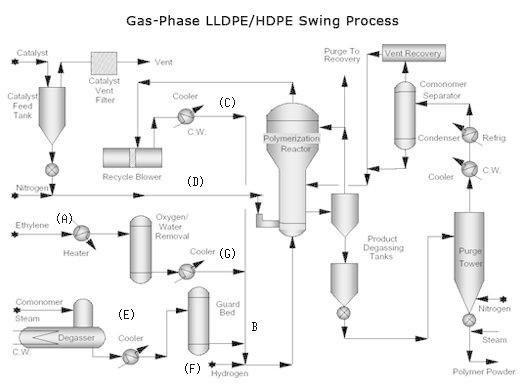
\includegraphics[width=0.8\textwidth,clip]{./Pics/hdpe_production_img2.jpg}
     \caption{HDPE fluxogram}\label{HDPE_Plant}
  \end{center}
\end{figure}

Systems that will be investigated are:
\begin{enumerate}[A.]
  \item {\bf Gaseous Ethylene Stream:} prior to the removal of water and oxygen at the pressure vessel, gaseous ethylene $\left(\text{XX}^{\circ}\text{C, A}\right)$ is heated up in a finned tube cross flow heat exchanger (Fig.~\ref{HE_FlowPastHeatedCyclinder}, bottom). In order to support the design of such heat exchanger, specific technical information with respect to flow dynamics and heat transfer need to be obtained.
     \begin{enumerate}[i)]
        \item\label{1a} Flow past a heated cylinder: In order to obtain the appropriate parameters for the design of such heat exchanger, a simplified 2D model involving ethylene gas flow past a heated cylinder (Fig.~\ref{HE_FlowPastHeatedCyclinder}, top) can be used to obtain information about drag forces and heat transfer (solid-fluid and fluid-fluid) that can later be used in the design and optimisation of the whole heat exchanger. 
        \item\label{1b} Flow past a bank of heated cylinders: With the experience gained in (\ref{1a}), it is important to investigate the drag and heat transfer mechanisms in a bank of heated cylinders, i.e., the impact of such set of obstacles in the flow dynamics.
        \item\label{1c} Cross-flow heat exchanger (see \href{https://www.youtube.com/watch?v=-03gO3UwFeA}{https://www.youtube.com/watch?v=-03gO3UwFeA}): After the preliminary study (\ref{1a}-\ref{1b}) wrt optimal configuration of bank of heated cylinders, extend the model to 3D simulation and investigate flow dynamics and heat transfer rate.
     \end{enumerate}

     {\bf Tasks:}
     \begin{itemize}
        \item Initial geometry, mesh (unstructured) and set-up for 2D configurations described in \ref{1a}-\ref{1b};
        \item Gas compressibility assumptions: incompressible and compressible using PR-EOS;
        \item Investigation of drag around the cylinder(s) and the impact in the induced heat diffusion;
        \item Investigation of turbulence induced by the cylinder(s) through different models;
        \item Heat transfer efficiency in the \ref{1c}, temperature gradient in ethylene and oil (internal flow fluid) streams;
        \item Maybe optimal design for the heat exchanger.
     \end{itemize}

     \begin{figure}[h]
         \vbox{ \hbox{\hspace{1cm}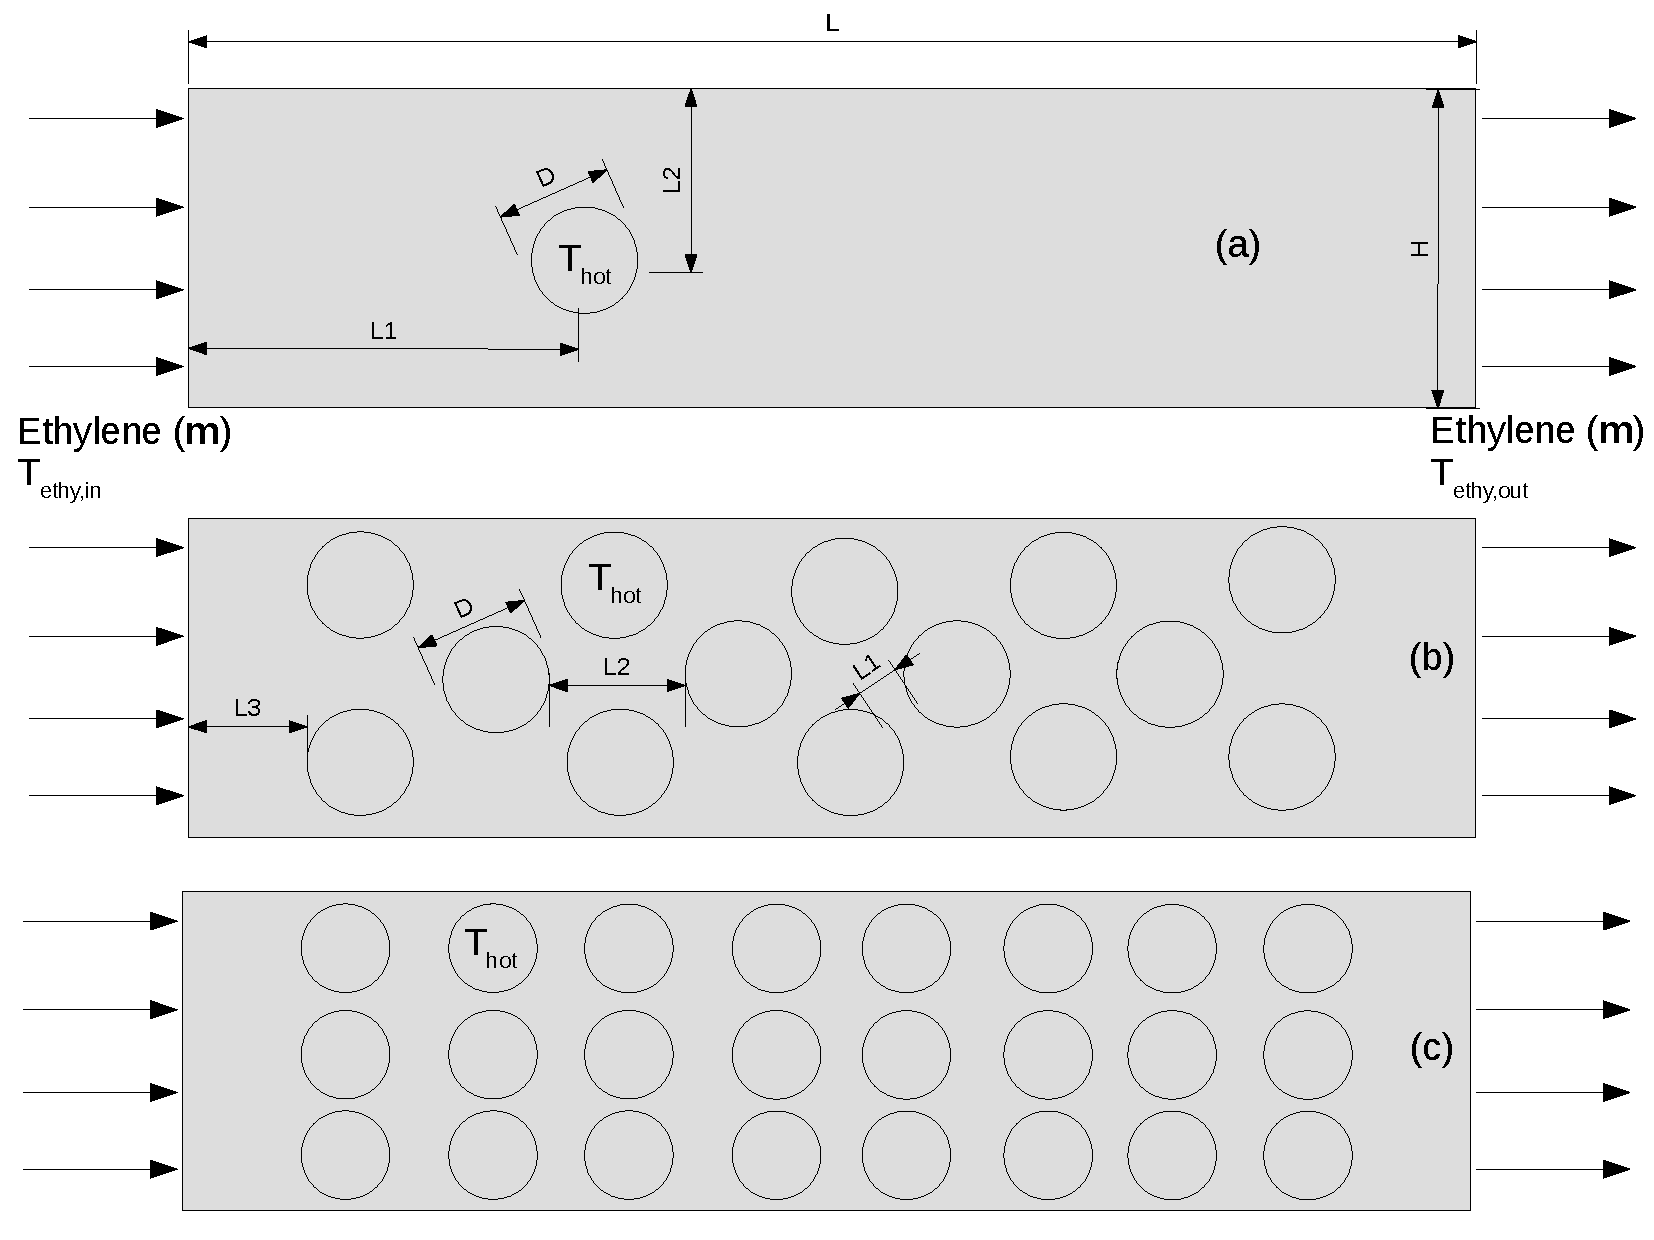
\includegraphics[width=0.7\textwidth,clip]{./Pics/HeatExchanger_2D.pdf}}
                \hbox{\hspace{3cm}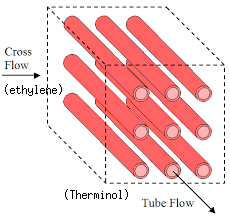
\includegraphics[width=0.5\textwidth,clip]{./Pics/HE_Finned.png}}}
         \caption{Flow past (heated) cylinder and banks of (heated) cylinders (top/middle). Cross-flow heat exchanger (bottom). }\label{HE_FlowPastHeatedCyclinder}
     \end{figure}

%%%
  \item {\bf Design of a Manifold Pipeline System:} four gaseous streams (B) are mixed before the polymerisation at the reactor in a hydraulic pipeline (Fig.~\ref{ManifoldPipeline}). The streams are:
     \begin{itemize}
        \item Ethylene (A) at XX$^{\circ}$C $\left(\dot{m}_{\text{ethyl}} = YY \text{kg.s}^{-1}\right)$;
        \item Hydrogen (F) at XY$^{\circ}$C $\left(\dot{m}_{\text{H}_{2}} = ZZ \text{kg.s}^{-1}\right)$;
        \item 2-Butene (comonomer, E) at XZ$^{\circ}$C $\left(\dot{m}_{\text{2-butene}} = ZY\right)$;
        \item Recycled (C, i.e., mixture of the above streams with composition of 15/60/25$\%$ in weight) at YZ$^{\circ}$C $\left(\dot{m}_{\text{rec}} = YX \text{kg.s}^{-1}\right)$.
     \end{itemize}
     
     {\bf Tasks:} The distance from the pre-processing units (A, C, E and F) to the reactor is of XX m and the reactor is placed in a platform at a height of YY m from the soil. You should design a manifold pipeline considering:
     \begin{itemize}
        \item Assume all pipelines are insulated and no heat is lost to the environment;
        \item Mesh analysis;
        \item The gaseous mixture should be injected into the polymerisation reactor at uniform temperature of $\left(kk\pm 5^{\circ}\text{C}\right)$. If the temperature resulting from the mixing does not reach the target, you may use an external heater (i.e., either prescribed heater temperature or flux);
        \item Turbulence models in the manifold pipeline system;
        \item Determine the optimal configuration for the manifold system that leads to the smallest pressure drop.
     \end{itemize}
     
     
     
    

     \begin{figure}[h]
         \vbox{ \hbox{\hspace{1cm}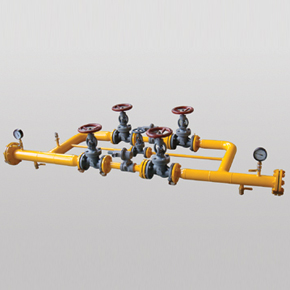
\includegraphics[width=0.7\textwidth,clip]{./Pics/ManifoldPipeline1.jpg}}
                \hbox{\hspace{3cm}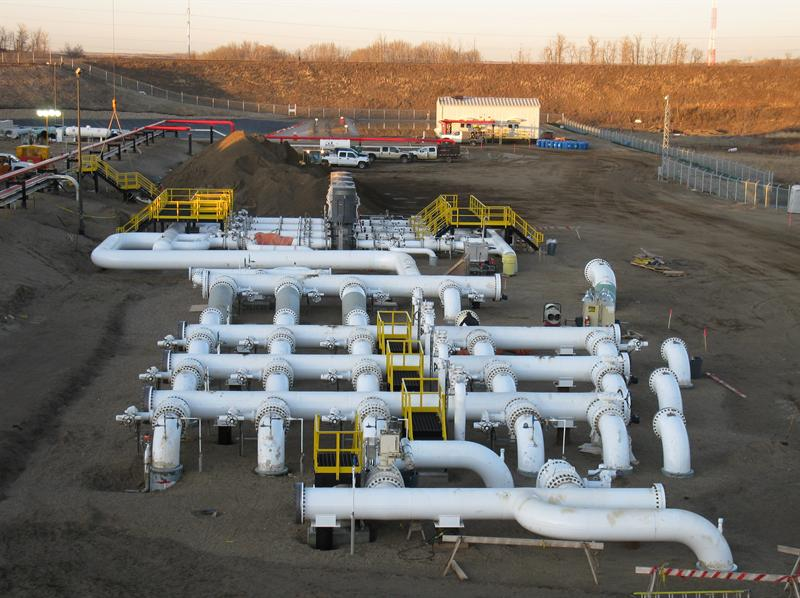
\includegraphics[width=0.5\textwidth,clip]{./Pics/ManifoldPipeline2.jpg}}}
         \caption{Manifold hydraulic pipeline (mixing of gases). }\label{ManifoldPipeline}
     \end{figure}


\end{enumerate}






\clearpage
\begin{center}
\Large{\bf Deliverables}
\end{center}
\begin{enumerate}[1)]
  \item Write a report containing:
  \begin{enumerate}
    \item Summary of {\bf all simulation set-ups} including,
       \begin{enumerate} [(a)]
          \item Initial and boundary conditions (for each simulation);
          \item Mesh information/quality;
          \item Numerical schemes (i.e., solution methods) and sub-models used.
       \end{enumerate}
    \item Summary of the numerical results (incl. figures displaying the data), findings, interpretation and \underline{analysis} along with concluding remarks.
  \end{enumerate}
  
  \item Report should contain no more than (\underline{maximum}) 8 pages including bibliography and appendices (if any) -- see attached example;

\item {\bf Prepare the report as \underline{PDF file} and submit it through {\it Turnitin} (with the appropriate plagiarism cover sheet) by Friday, November 24$^{\text{th}}$ 2017, noon at the latest. Also, submit a hard-copy of the report to the UG office by November 24$^{\text{th}}$, 15.00h.}
%
%\item Feedback will be provided on December YY$^{th}$ 2015.
%
\item Penalties for late or non-submission are as follows:
\begin{enumerate}%[(a)]
  \item Up to one week late, 2 CGS points deducted;
  \item Up to two weeks late, 3 CGS point deducted;
  \item More than two weeks late no marks awarded.
\end{enumerate}
If late or non-submission is due to medical or other circumstances out with your control you must submit a medical certificate or other formal evidence to the UG Office as soon as is practicable but no later than the end of Revision Week.

\item Note that the submitted work is part of the continuous assessment which will contribute 40$\%$ to your EG501V mark.

\end{enumerate}

\end{document}
